\title{คาบเรียนที่ 15: ความยาวส่วนโค้ง }
\frame{\titlepage}

\begin{frame}
\frametitle{ทบทวน}
เรานิยามปริพันธ์จำกัดเขต
\[ \int_a^b f(x) \, dx\]
เป็นพื้นที่ใต้เส้นโค้ง $y = f(x)$ เหนือแกน $x$ ด้วยการตีความว่า
\[ f(x) \, dx \]
คือพื้นที่สี่เหลี่ยมผืนผ้า ที่มีความสูงเป็น $f(x)$ และความกว้างฐานเป็น $dx$
\end{frame}

\begin{frame}
\frametitle{เนื้อหาใหม่}
ถ้าเราเปลี่ยนความหมายของฟังก์ชัน $f(x)$ เป็นอย่างอื่น จะทำให้เราสามารถใช้ปริพันธ์จำกัดเขตในการคำนวณค่าต่าง ๆ โดยเราจะศึกษาการประยุกต์ 4 รูปแบบด้วยกัน ได้แก่
\tableofcontents
\end{frame}

%%%%%%%%%
\section[มวลของเส้นลวด]{มวลของเส้นลวด}
\frame{\sectionpage}
%%%%%%%%%%%

\begin{frame}
\frametitle{การหามวลของเส้นลวด}
แทนที่เราจะมอง $f(x)$ เป็นเส้นโค้ง เราสามารถมอง $f(x)$ เป็นความหนาแน่นของเส้นลวด ณ จุด $x$ แทนได้ โดยสมมติว่าเส้นลวดมีความบางมาก
\addfig{0.7}{int_applied_wire_intro}{เส้นลวดที่มีความหนาแน่นในแต่ละจุดไม่เท่ากัน}{}
\end{frame}

\begin{frame}
\frametitle{สูตรมวลของเส้นลวด}
ในทางฟิสิกส์ เราจะแทนความหนาแน่นด้วยตัวแปร $\rho$ (อ่านว่าโร) ฉะนั้นเราจึงเปลี่ยนชื่อฟังก์ชันใหม่ ดังนี้
\begin{thm}{}{}
กำหนดให้ $\rho(x)$ เป็นฟังก์ชันความหนาแน่นของเส้นลวดบาง ณ จุด $x$ และให้มวลของเส้นลวดบนช่วง $x \in [a,b]$ มีค่าเท่ากับ $M$ แล้วจะได้ว่า
\begin{equation} \label{eq:int_applied_mass}
M = \int_a^b \rho(x) \, dx
\end{equation}
\end{thm}
\end{frame}


\begin{frame}[t] 
\begin{ex} 
จงหามวลของเส้นลวดบางที่มีฟังก์ชันความหนาแน่นเป็น $\rho(x) = x^3+x$ บนช่วง $x \in [0,2]$
\end{ex} 
\begin{sol}
เนื่องจากโจทย์ระบุข้อมูลทุกอย่างมาให้แล้ว ฉะนั้นเราสามารถใช้สมการ \eqref{eq:int_applied_mass} ได้ทันที จะได้
\begin{eq*}
M = \int_a^b \rho(x) \, dx &=& \int_0^2 (x^3+x) \, dx  \\
&=& \left( \frac{1}{4}x^4 + \frac{1}{2}x^2 \right) \Big|_0^2 \\
&=& \left( \frac{1}{4} (2)^4 + \frac{1}{2} (2)^2\right) - \left( \frac{1}{4} (0)^4 + \frac{1}{2} (0)^2\right) \\
&=& (4+2) - (0+0) = 6
\end{eq*}
\end{sol}
\end{frame}

%%%%%%%%%
\section{ความยาวเส้นโค้ง}
\frame{\sectionpage}
%%%%%%%%%%%

\begin{frame}
\frametitle{ที่มาของสูตร}
กำหนดเส้นโค้ง $y=f(x)$ จาก $x=a$ ถึง $x=b$ \pa แล้วเราสามารถหาความยาวส่วนโค้งได้ \pa ด้วยการกำหนดจุดบนเส้นโค้งและลากเส้นตรงเชื่อมจุดเข้าด้วยกัน \pa
\begin{figure}[h!]
\centering
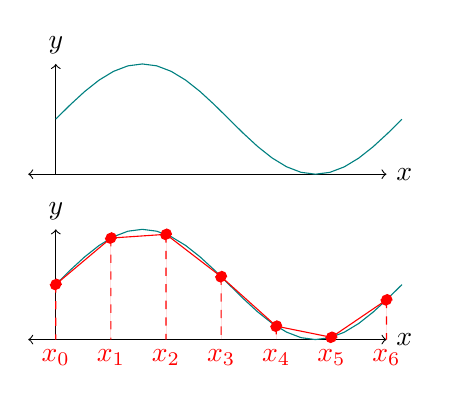
\begin{tikzpicture}[scale = 0.7]
\draw[<->] (-0.5,0) -- (6,0) node[right] {$x$};
\draw[->] (0,0) -- (0,2) node[above] {$y$};
\draw[teal, domain = 0:6.28] plot (\x, {1+sin(\x r)});
\begin{scope}[yshift = -3cm]
\draw[<->] (-0.5,0) -- (6,0) node[right] {$x$};
\draw[->] (0,0) -- (0,2) node[above] {$y$};
\draw[teal, domain = 0:6.28] plot (\x, {1+sin(\x r)});
\foreach \x in {0,1,2,3,4,5}
{
	\filldraw[red, dashed] (\x, {1+sin(\x r)}) circle (0.1cm) -- (\x,0) node[below] {$x_{\x}$};
	\draw[red] (\x, {1+sin(\x r)}) -- ({\x+1}, {1+sin((\x+1) r)});
}
\filldraw[red, dashed] (6, {1+sin(6 r)}) circle (0.1cm) -- (6,0) node[below] {$x_6$};
\end{scope}
\end{tikzpicture}
\caption{การประมาณความส่วนโค้ง ด้วยเส้นตรงที่แบ่งเป็นช่วง ๆ}
\end{figure}
\end{frame}

\begin{frame}
พิจารณาเส้นตรงที่เชื่อมจุดสองจุด ได้แก่ จุด $(x_0, f(x_0))$ และจุด $(x_1, f(x_1))$ \pa

\begin{figure}[h!]
\centering
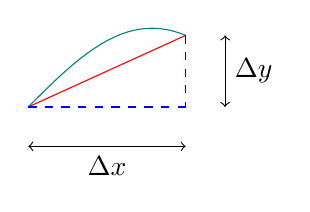
\begin{tikzpicture}
\axes{-0.5}{2.5}{-0.5}{2}
\draw[teal, domain = 0:2] plot (\x, {1+sin(\x r)});
\draw[red] (0, {1+sin(0 r)}) -- (2, {1+sin(2 r)});
\draw[blue, dashed] (0, {1+sin(0 r)}) --+ (2,0);
\draw[<->] (0, {0.5+sin(0 r)}) --+ (2,0) node[below, pos = 0.5] {$\Delta x$};
\draw[blue, dashed] (2, {1+sin(2 r)}) -- (2,{1+sin(0 r)});
\draw[<->] (2.5, {1+sin(2 r)}) -- (2.5,{1+sin(0 r)}) node[right, pos = 0.5] {$\Delta y$};
\end{tikzpicture}
\caption{ความสัมพันธ์ระหว่างส่วนของเส้นตรงระหว่างสองจุด และค่า $\Delta x$ และ $\Delta y$}
\label{}
\end{figure}

เส้นตรงนี้ คือเส้นตรงข้ามมุมฉากในสามเหลี่ยมที่มีความกว้าง $x_1 - x_0 = dx$ และความสูง $f(x_1) - f(x_0) = dy$ 
\end{frame}

\begin{frame}
จากนั้นเราสามารถใช้ทฤษฎีบทปิทากอรัส เพื่อหาความยาวเส้นตรงได้เป็น \pa
\[\sqrt{(dx)^2 + (dy)^2}\]
\pa ซึ่งสามารถเขียนใหม่ได้ดังนี้
\[\sqrt{(dx)^2 + (dy)^2} = \sqrt{(dx)^2 + (dx)^2\left( \frac{dy}{dx} \right)^2} = \sqrt{1 + \left(\frac{dy}{dx}\right)^2} \, dx\]
\pa ดังนั้น ความยาวเส้นตรงรวมกันมีค่าเท่ากับ
\[\sum \sqrt{1 + \left(\frac{dy}{dx}\right)^2} \, dx \]
\end{frame}

\begin{frame}
\pa และเมื่อเราแบ่งช่วงย่อยให้มากขึ้นเรื่อย ๆ จนจำนวนช่วงย่อยเข้าใกล้อนันต์ จึงได้สูตร
\[L = \int_a^b \sqrt{1 + \left(\frac{dy}{dx}\right)^2} \, dx \]
\begin{figure}[h!]
\centering
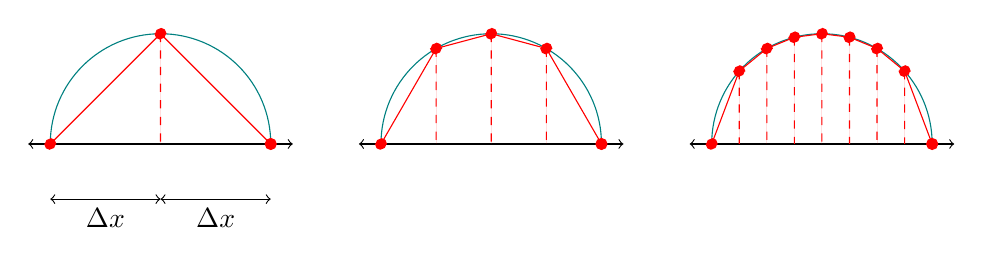
\begin{tikzpicture}[scale = 1.4]
\begin{scope}[xshift = 0cm]
\draw[<->] (-1.2,0) -- (1.2,0);
\draw[teal] (1,0) arc [start angle = 0, end angle = 180, radius = 1];
\foreach \x in {-1,0}
{
	\filldraw[red, dashed] (\x, {sqrt(1-(\x*\x))}) circle (0.05cm) -- (\x,0);
	\draw[red] (\x, {sqrt(1-(\x*\x))}) -- ({\x+1}, {sqrt(1-(\x+1)*(\x+1)))});
	\draw[<->] (\x, -0.5) --+ (1,0) node[below, pos = 0.5] {$\Delta x$};
}
\filldraw[red] (1, 0) circle (0.05cm);
\end{scope}
\begin{scope}[xshift = 3cm]
\draw[<->] (-1.2,0) -- (1.2,0);
\draw[teal] (1,0) arc [start angle = 0, end angle = 180, radius = 1];
\foreach \x in {-1,-0.5,0,0.5}
{
	\filldraw[red, dashed] (\x, {sqrt(1-(\x*\x))}) circle (0.05cm) -- (\x,0);
	\draw[red] (\x, {sqrt(1-(\x*\x))}) -- ({\x+0.5}, {sqrt(1-(\x+0.5)*(\x+0.5)))});
}
\filldraw[red] (1, 0) circle (0.05cm);
\end{scope}
\begin{scope}[xshift = 6cm]
\draw[<->] (-1.2,0) -- (1.2,0);
\draw[teal] (1,0) arc [start angle = 0, end angle = 180, radius = 1];
\foreach \x in {-1,-0.75,-0.5,...,0.75}
{
	\filldraw[red, dashed] (\x, {sqrt(1-(\x*\x))}) circle (0.05cm) -- (\x,0);
	\draw[red] (\x, {sqrt(1-(\x*\x))}) -- ({\x+0.25}, {sqrt(1-(\x+0.25)*(\x+0.25)))});
}
\filldraw[red] (1, 0) circle (0.05cm);
\end{scope}
\end{tikzpicture}
\caption{การประมาณความยาวส่วนโค้ง โดยใช้จำนวนช่วงย่อยมากขึ้นเรื่อย ๆ}
\end{figure}
\end{frame}


\begin{frame}
\frametitle{สูตรหาความยาวเส้นโค้ง}
\begin{thm}{}{}
กำหนดฟังก์ชัน $f(x)$ เป็นฟังก์ชันต่อเนื่องและหาอนุพันธ์ได้บนช่วง $[a,b]$ แล้วความยาวส่วนโค้งของกราฟ $y = f(x)$ จาก $x =a$ ถึง $x=b$ มีค่าเท่ากับ
\begin{equation} \label{eq:int_applied_curve_length}
L= \int_a^b \sqrt{1 + \left(\dyx\right)^2} \, dx
\end{equation}
\end{thm}
เราสามารถย่อเป็น $\int_a^b \sqrt{1 + (f\,')^2} \, dx$ ก็ได้ 
\end{frame}

 
\begin{frame}[t] 
\begin{ex} 
จงหาความยาวเส้นโค้งของกราฟ $y = 2x+1$ บนช่วง $[0,4]$ 
\end{ex} 
\begin{sol}
อนุพันธ์ของฟังก์ชันคือ $\dyx = 2$ ฉะนั้น ความยาวส่วนโค้งบนช่วง $[0,4]$ มีค่าเท่ากับ \pa
\begin{eq*}
\int_a^b \sqrt{1 + \left(\dyx\right)^2} \, dx \pa &=& \int_0^4 \sqrt{1 + (2)^2} \, dx \\ \pa
&=& \int_0^4 \sqrt{5} \, dx \\ \pa
&=& \sqrt{5} x \Big|_0^4 \\ \pa
&=& 4\sqrt{5}
\end{eq*}
\end{sol}
\end{frame}


 
\begin{frame}[t] 
\begin{ex} 
จงหาความยาวเส้นโค้งของกราฟ $y = \frac{2}{3}x^{3/2}$ บนช่วง $[0,1]$ 
\end{ex} 
\begin{sol}
อนุพันธ์ของฟังก์ชันคือ $\dyx = \sqrt{x}$ \pa ฉะนั้น ความยาวส่วนโค้งบนช่วง $[0,1]$ มีค่าเท่ากับ \pa
\begin{eq*}
\int_a^b \sqrt{1 + \left(\dyx\right)^2} \, dx \pa &=& \int_0^1 \sqrt{1 + \left( \sqrt{x}\right)^2} \, dx \\ \pa
&=& \int_0^1 \sqrt{1 + x } \, dx
\end{eq*}
\pa เราต้องใช้เทคนิคการแทนค่า $u$ ในการหาปริพันธ์นี้
\end{sol}
\end{frame}

\begin{frame}
\begin{sol} (ต่อ)
กำหนดให้ $ u =1 + x$ \pa จะได้ $du = dx$ \pa ดังนั้น
\begin{eq*}
\int \sqrt{1 + x} \, dx \pa &=& \int \sqrt{u} \, du \\ \pa
&=& \frac{2}{3}u^{3/2} + C \\ \pa
&=& \frac{2}{3} \left(1 + x \right)^{3/2} + C
\end{eq*}
ฉะนั้น ความยาวส่วนโค้งมีค่าเท่ากับ
\begin{eq*}
\int_0^1 \sqrt{1 + x } \, dx &=& \left( \frac{2}{3} \left(1 + x \right)^{3/2} \right) \Big|_0^1 \\ \pa
&=& \frac{2}{3} \left(1 + 1 \right)^{3/2} - \frac{2}{3} \left(1 + 0 \right)^{3/2} \\ \pa
&=& \frac{2}{3} ( 2^{3/2} - 1 ) = \frac{2}{3} (2\sqrt{2} - 1) \pa
\end{eq*}
\end{sol}
\end{frame}

%%%%%%%%%
\section[ปริมาตรพื้นที่ภาคตัด]{ปริมาตรของรูปทรงตันซึ่งหาพื้นที่ภาคตัดได้}
\frame{\sectionpage}
%%%%%%%%%%%

\begin{frame}
\frametitle{ที่มาของการหาปริมาตร}
พิจารณารูปทรงตันสามมิติ ที่เราต้องการหาปริมาตร เราสามารถแบ่งออกเป็นรูปทรงขนาดเล็กได้ โดยใช้ระนาบตัดออกเป็นส่วน ๆ เข้าด้วยกัน
\addfig{0.7}{integral_volume_slice_concept}{การเฉือนรูปทรงตันด้านซ้าย จะได้พื้นที่หน้าตัดออกมาดังภาพด้านขวา}{}
\end{frame}

\begin{frame}
ปริมาตรของรูปที่ถูกตัดออกคือ
\[\text{พื้นที่หน้าตัด } \cdot \text{ ความกว้าง } = A \cdot dx\]
ถ้าเรากำหนดฟังก์ชัน $A(x)$ เท่ากับพื้นที่หน้าตัดที่เกิดจากการตัดรูปทรงที่จุด $x$ จะได้ปริมาตรเป็น
\[ A(x) \, dx\]
ซึ่งเมื่อรวมปริมาตรทั้งหมดเข้าด้วยกัน และหาลิมิตเมื่อจำนวนชิ้นที่ตัดเข้าใกล้อนันต์ จะได้ปริมาตรเป็น
\[V = \int_a^b A(x) \, dx\]
\end{frame}

\begin{frame}
\frametitle{สูตรปริมาตรของรูปทรงตันซึ่งหาพื้นที่ภาคตัดได้}
\begin{thm}{}{}
กำหนดทรงตัน $S$ ที่อยู่ระหว่างระนาบ $x=a$ และ $x=b$ ถ้าพื้นที่ผิวของรอยตัดของ $S$ ที่จุด $x$ ใด ๆ มีค่าเท่ากับ $A(x)$ แล้วปริมาตรของทรงตันมีค่าเท่ากับ
\begin{equation} \label{eq:int_applied_volume_slice}
V = \int_a^b A(x) \, dx
\end{equation}
\end{thm}
\end{frame}


\begin{frame}[t] 
\begin{ex} 
จงหาสูตรปริมาตรของปิรามิดฐานสี่เหลี่ยมจัตุรัส ที่มีความสูง $h$ และความกว้างฐาน $a$
\end{ex} 
\begin{sol}
เราสามารถวาดรูปปิรามิดในแนวแกน $x$ ได้ดังนี้
\addfig{0.9}{integral_volume_slice_ex1}{ปิรามิดความสูง $h$ และความกว้างฐาน $a$ ที่มีจุดยอดที่จุด $(0,0)$ และฐานที่ผ่านจุด $(a,0)$}{}
\end{sol}
\end{frame}

\begin{frame}[t]
\begin{sol} (ต่อ)
พื้นที่เฉือนของรูปสี่เหลี่ยมจัตุรัสมีค่าเท่ากับ
\[A(x) = s^2 = \frac{a^2}{h^2} x^2\]
ฉะนั้น ปริมาตรของปิรามิดมีค่าเท่ากับ
\begin{eq*}
V = \int_0^h A(x) \, dx &=& \int_0^h \frac{a^2}{h^2}x^2 \, dx \\
&=& \frac{a^2}{h^2} \int_0^h x^2 \, dx \\
&=& \frac{a^2}{h^2} \left( \frac{1}{3} x^2 \right) \Big|_0^h \\
&=& \frac{a^2}{h^2}\left( \frac{1}{3}h^3 - 0 \right) \\
&=& \frac{1}{3}a^2 h
\end{eq*}
\end{sol}
\end{frame}

%%%%%%%%%
\section[หมุนพื้นที่โดยวิธีจาน]{ปริมาตรของรูปทรงตันที่เกิดจากการหมุนพื้นที่โดยวิธีจาน \\ (Disk and washer method)}
\frame{\sectionpage}
%%%%%%%%%%%

\begin{frame}
\frametitle{ที่มา}
กำหนดเส้นโค้ง $y=f(x)$ เราสามารถหาบริเวณใต้เส้นโค้ง ระหว่าง $x=a$ ถึง $x=b$ ได้ดังนี้
\addfig{0.7}{integral_volume_disk_concept1}{บริเวณใต้เส้นโค้ง}{}
\end{frame}

\begin{frame}
ถ้าเราติดกาวบริเวณนี้เข้ากับแกน $x$ และจับแกน $x$ หมุนรอบโดยที่ยังคงให้แกน $x$ อยู่ตำแหน่งเดิม จะเกิดเป็นรูปทรงดังนี้
\addfig{0.7}{integral_volume_disk_concept2}{การหมุนบริเวณรอบแกน $x$}{}
\end{frame}

\begin{frame}
สุดท้าย ถ้าเราหมุนจนครบ 360 องศา (หรือเป็นมุม $2\pi$) จะทำให้เกิดทรงตันปิดขึ้นมา
\addfig{0.7}{integral_volume_disk_concept3}{รูปทรงที่เกิดจากการหมุนรอบแกน $x$ ครบรอบ}{}
\end{frame}

\begin{frame}
สังเกตว่า รูปทรงตันปิดที่เกิดจากการหมุนนี้ เราสามารถเฉือนออกเป็นรูปจานได้ โดยพื้นที่ผิวของจานที่เฉือน ณ จุด $x$ มีค่าเท่ากับ
\[ \pi (r)^2 = \pi (f(x))^2\]
ฉะนั้นปริมาตรของจานคือ $\pi (f(x))^2 \, dx$ และทำให้ได้สูตรปริมาตรของรูปที่เกิดจากการหมุนทั้งรูปเป็น
\[V = \int_a^b \pi (f(x))^2 \, dx \]
\end{frame}

\begin{frame}
\frametitle{สูตรปริมาตรของรูปทรงตันที่เกิดจากการหมุนพื้นที่โดยวิธีจาน}
\begin{thm}{}{}
กำหนดทรงตัน $S$ ที่เกิดจากการหมุนบริเวณที่ล้อมรอบด้วยเส้นโค้ง $y = f(x), x = a, x = b$ และแกน $x$ รอบแกน $x$ แล้วปริมาตรของทรงตันมีค่าเท่ากับ
\begin{equation} \label{eq:int_applied_volume_disk_x}
V = \int_a^b \pi (f(x))^2 \, dx 
\end{equation}
\end{thm}
\end{frame}




\begin{frame}[t] 
\begin{ex} 
จงหาปริมาตรที่เกิดจากการหมุนพื้นที่ซึ่งล้อมรอบด้วยเส้นโค้ง $y=x^2, x=2$ และแกน $x$ รอบแกน $x$
\end{ex} 
\begin{sol}
โจทย์ไม่ได้ให้ขอบเขตด้านซ้ายมา แต่จากการวาดกราฟพบว่า $y=x^2$ ตัดแกน  $x$ ที่ $x=0$ ฉะนั้นขอบเขตด้านซ้ายคือ $a=0$ 

จากนั้น เราจึงใช้สูตร \eqref{eq:int_applied_volume_disk_x} ได้ทันที \pa ฉะนั้น ปริมาตรมีค่าเท่ากับ
\begin{eqnarray*}
V = \iii{0}{2}{\pi (x^2)^2} \pa &=& \iii{0}{2}{\pi x^4} \\
\pa &=& \pi \frac{1}{5} x^5 \Big|_0^2 \\
\pa &=& \pi \frac{1}{5} 2^5 - \pi \frac{1}{5} 0^5 \\
\pa &=& \frac{32}{5} \pi
\end{eqnarray*}
\end{sol}
\end{frame}

\begin{frame}
\addfig{0.6}{int_applied_disk1}{ตัวอย่างรูปทรงตัน ที่เกิดจากการหมุนบริเวณสีฟ้ารอบแกน $x$}{}
\end{frame}


\begin{frame}[t] 
\begin{ex} 
จงหาปริมาตรทรงสามมิติ ที่เกิดจากการหมุนบริเวณ $R$ รอบแกน $x$ โดย $R$ คือบริเวณที่ปิดล้อมด้วยเส้นโค้ง $y=2x$, เส้นตรง $x=1$, เส้นตรง $x=4$ และแกน $x$
\end{ex}
\begin{sol}
เนื่องจากโจทย์ให้ข้อมูลมาครบถ้วนแล้ว เราจึงสามารถใช้สูตร \eqref{eq:int_applied_volume_disk_x} ได้ทันที ฉะนั้น ปริมาตรมีค่าเท่ากับ
\begin{eqnarray*}
V = \iii{1}{4}{\pi (2x)^2} \pa &=& \iii{1}{4}{\pi 4x^2} \\
\pa &=& \pi \frac{4}{3} x^3 \Big|_1^4 \\
\pa &=& \pi \frac{4}{3} 4^3  - \pi \frac{4}{3} 1^3 \\
\pa &=& \pi \frac{4}{3} (64-1) \\
\pa &=& 84 \pi
\end{eqnarray*}
\end{sol}
\end{frame}

\begin{frame}
\addfig{0.6}{int_applied_disk2}{ตัวอย่างรูปทรงตัน ที่เกิดจากการหมุนบริเวณสีฟ้ารอบแกน $x$}{}
\end{frame}

\begin{frame}
\frametitle{การหมุนรอบเส้นตรง $y=c$}
เราไม่จำเป็นต้องสร้างทรงสามมิติโดยการหมุนรอบแกน $x$ เสมอไป ถ้าโจทย์กำหนดเส้นตรง $y=c$ มาให้ เราสามารถหาปริมาตรของทรงสามมิติได้ดังนี้
\begin{thm}{}{}
กำหนดทรงตัน $S$ ที่เกิดจากการหุนบริเวณที่ล้อมรอบด้วยเส้นโค้ง $y = f(x), x = a, x = b$ และเส้นตรง $y=c$ รอบแกน $x$ แล้วปริมาตรของทรงตันมีค่าเท่ากับ
\begin{equation} \label{eq:int_applied_volume_disk_another_line}
V = \int_a^b \pi (f(x)-c)^2 \, dx 
\end{equation}
\end{thm}
ข้อสังเกต: เนื่องจากแกน $x$ กำหนดด้วยเส้นตรง $y=0$ ดังนั้นเราจึงสามารถใช้สูตรนี้ได้เช่นกัน
\end{frame}

\begin{frame}
\addfig{0.6}{int_applied_disk4}{ตัวอย่างรูปทรงตัน ที่เกิดจากการหมุนบริเวณสีฟ้ารอบเส้นตรง $y=1$}{}
\end{frame}

\begin{frame}
\frametitle{การหมุนรอบแกน $y$}
เราไม่จำเป็นต้องสร้างทรงสามมิติโดยการหมุนรอบแกน $x$ เสมอไป ถ้าโจทย์กำหนดเส้นตรง $y=c$ มาให้ เราสามารถหาปริมาตรของทรงสามมิติได้ดังนี้
\begin{thm}{}{}
กำหนดทรงตัน $S$ ที่เกิดจากการหมุนบริเวณที่ล้อมรอบด้วยเส้นโค้ง $x = w(y)$, $y = a$, $y = b$ และแกน $y$ รอบแกน $y$ แล้วปริมาตรของทรงตันมีค่าเท่ากับ
\begin{equation} \label{eq:int_applied_volume_disk_y}
V = \int_a^b \pi (w(y))^2 \, dy 
\end{equation}
\end{thm}
\end{frame}

\begin{frame}
\addfig{0.8}{int_applied_disk5}{ตัวอย่างรูปทรงตัน ที่เกิดจากการหมุนบริเวณสีฟ้ารอบแกน $y$}{}
\end{frame}

%%%%%%%%%
\section[หมุนพื้นที่โดยวิธีเปลือกทรงกระบอก]{ปริมาตรของรูปทรงตันที่เกิดจากการหมุนพื้นที่โดยวิธีเปลือกทรงกระบอก \\ (Cylindrical shell method)}
\frame{\sectionpage}
%%%%%%%%%%%

\begin{frame}
\frametitle{ที่มา}
สมมติว่า แทนที่จะหมุนรอบแกน $x$ เราสามารถหมุนรอบแกน $y$ แทนได้ โดยรูปที่ได้จะออกมาคล้ายรูปทรงกระบอก
\addfig{0.7}{integral_volume_shell_concept1}{รูปเปลือกทรงกระบอกที่เกิดจากการหมุนบริเวณรอบแกน $y$}{}
\end{frame}

\begin{frame}
หลักการหาปริมาตรคือ เริ่มจากการแบ่งรูปคล้ายทรงกระบอก ออกเป็นเปลือกทรงกระบอก
\addfig{0.9}{integral_volume_shell_concept2}{บริเวณใต้เส้นโค้ง}{}
\end{frame}

\begin{frame}
จากนั้น เราสามารถประมาณปริมาตรของเปลือกทรงกระบอกได้ด้วยการคลี่ออกมา คล้ายรูปทรงสี่เหลี่ยมผืนผ้าดังภาพ
\addfig{0.9}{integral_volume_shell_concept3}{บริเวณใต้เส้นโค้ง}{}
\end{frame}

\begin{frame}
ปริมาตรของเปลือกทรงกระบอกที่ถูกคลี่ออกมาเป็นทรงสี่เหลี่ยมผืนผ้าแล้ว มีค่าประมาณ
\[ \text{ กว้าง x สูง x ฐาน} = 2 \pi x f(x) \, dx\]
ฉะนั้น เมื่อรวมปริมาตรของเปลือกทรงกระบอกทั้งหมดเข้าด้วยกัน จึงได้สูตรการปริมาตรเป็น
\[V = \int_a^b 2\pi x f(x) \, dx\]
\end{frame}

\begin{frame}
\frametitle{สูตรปริมาตรของรูปทรงตันที่เกิดจากการหมุนพื้นที่โดยวิธีเปลือกทรงกระบอก}
\begin{thm}{}{}
กำหนดทรงตัน $S$ ที่เกิดจากการหมุนบริเวณที่ล้อมรอบด้วยเส้นโค้ง $y=f(x)$, $x = a$, $x=b$ และแกน $x$ โดยหมุนรอบแกน $y$ แล้วปริมาตรของทรงตันมีค่าเท่ากับ
\begin{equation} \label{eq:int_applied_volume_shell}
V = \int_a^b 2\pi x f(x) \, dx
\end{equation}
\end{thm}
\end{frame}


\begin{frame}[t] 
\begin{ex} 
จงหาปริมาตรที่เกิดจากการหมุนพื้นที่ซึ่งล้อมรอบด้วยเส้นโค้ง $y=\frac{1}{x}, x = 1, x=3$ และแกน $x$ รอบแกน $y$
\end{ex} 
\begin{sol}
สามารถใช้สูตรได้ทันที ได้
\begin{eq*}
V &=& \int_1^3 2 \pi x f(x) \, dx \\
&=& \int_2^3 2 \pi x \left( \frac{1}{x} \right) \, dx \\
&=& \int_1^3 2 \pi \, dx \\
&=& (2 \pi x) \Big|_1^3 = 4 \pi
\end{eq*}
\end{sol}
\end{frame}

\begin{frame}
\addfig{0.8}{integral_volume_shell_ex1}{รูปทรงตันที่เกิดจากการหมุนบริเวณ $R$}{}
\end{frame}